\section{Results and Interpretation Changes}
\label{sec:results}

Unless stated otherwise, comparisons refer to systems in their released configurations; deployment-sensitivity results are reported separately in the supplementary material and never redefine a system's native behaviour.

\subsection{Native-Capability Audit}
\label{sec:results_native}

Table~\ref{tab:t2v_audit} summarizes SNF-Bench measurements under released inference configurations at the two principal horizons, with all four reported in the supplementary material. The audited systems happen to share a deployment envelope---all seven generate $832\times480$ at $16$\,fps and all reach the $240$\,s horizon without modification to their released temporal policy---so no per-system configuration table is needed; where a system could not reach a horizon, the entry would be marked unsupported rather than populated with altered settings.

\begin{table}[!tb]
\centering
\scriptsize
\setlength{\tabcolsep}{2.6pt}
\begin{tabular}{lcccc}
\toprule
Method & fBD$\downarrow$ & NBF$\downarrow$ & MCFF E$\rightarrow$L & FP$\uparrow$ \\
\midrule
\multicolumn{5}{l}{\textit{60s horizon  ($n=23$)}} \\
CausVid & 8.08\,\tiny$\pm$3.15 & 9.27\,\tiny$\pm$4.14 & 2.87\,$\rightarrow$\,1.96 & 0.67\,\tiny$\pm$0.18 \\
Self-Forcing & 11.4\,\tiny$\pm$3.63 & 12.7\,\tiny$\pm$3.97 & 10.4\,$\rightarrow$\,2.54 & 0.44\,\tiny$\pm$0.22 \\
Infinite-Forcing & 7.75\,\tiny$\pm$3.84 & 3.65\,\tiny$\pm$0.88 & 1.17\,$\rightarrow$\,0.29 & 0.63\,\tiny$\pm$0.22 \\
Rolling-Forcing & 16.8\,\tiny$\pm$3.69 & 11.2\,\tiny$\pm$2.70 & 3.18\,$\rightarrow$\,1.57 & 0.75\,\tiny$\pm$0.29 \\
Reward-Forcing & 14.8\,\tiny$\pm$3.71 & 8.51\,\tiny$\pm$2.79 & 3.81\,$\rightarrow$\,0.80 & 0.49\,\tiny$\pm$0.18 \\
LongLive & 15.9\,\tiny$\pm$2.89 & 13.9\,\tiny$\pm$4.76 & 6.46\,$\rightarrow$\,2.41 & 0.75\,\tiny$\pm$0.28 \\
Causal-Forcing & 22.4\,\tiny$\pm$2.26 & 87.6\,\tiny$\pm$18.6 & 9.84\,$\rightarrow$\,7.21 & 0.83\,\tiny$\pm$0.31 \\
\midrule
\multicolumn{5}{l}{\textit{120s horizon  ($n=6$)}} \\
CausVid & 6.15 & 3.42 & 0.36\,$\rightarrow$\,0.52 & 1.06 \\
Self-Forcing & 21.2 & 6.80 & 4.85\,$\rightarrow$\,0.82 & 0.85 \\
Infinite-Forcing & 16.1 & 2.60 & 0.50\,$\rightarrow$\,0.32 & 0.64 \\
Rolling-Forcing & 23.8 & 10.6 & 3.33\,$\rightarrow$\,0.77 & 0.38 \\
Reward-Forcing & 20.0 & 11.6 & 2.05\,$\rightarrow$\,0.69 & 0.39 \\
LongLive & 22.5 & 9.66 & 5.10\,$\rightarrow$\,1.19 & 0.81 \\
Causal-Forcing & 21.8 & 130 & 10.5\,$\rightarrow$\,10.7 & 0.90 \\
\bottomrule
\end{tabular}
\caption{\textbf{Matched T2V checkpoint audit.} Public checkpoints are evaluated under one common four-step, guidance-$5.0$, six-frames-per-block, fixed-seed setting; results characterize this wrapper, not released inference procedures. $n$ is common within each horizon. Entries are prompt means $\pm$ half a percentile-bootstrap 95\% interval (10k resamples, fixed seed); $n<10$ panels show means only. MCFF-E$\rightarrow$L contextualizes the FP ratio. Marginal intervals are descriptive; separation claims use paired per-prompt bootstrap differences (Table~S3). DLR/DAR and aggregation sensitivity are in the supplement.}
\label{tab:t2v_audit}
\end{table}

\paragraph{Motion persistence.} Dynamic-region behavior is evaluated at the joint operating point $\bigl(\mathrm{MCFF}(\mathcal{L}),\,\mathrm{FP}\bigr)$, never FP alone: sustained flow requires non-trivial late motion \emph{and} high retention. Reporting MCFF-E beside MCFF-L makes the degenerate case visible---a system with negligible motion throughout cannot reach a high FP without also displaying a small MCFF-E.

\paragraph{Static--dynamic operating regimes.} Figure~\ref{fig:regimes_native} places each system in the static-drift--surviving-flow plane, exposing qualitatively different regimes---low-drift/low-motion, high-motion/high-drift, and low-drift/non-trivial-motion---without collapsing the axes into a scalar score. The two extremes are informative in opposite directions: Infinite-Forcing attains the lowest static drift of any audited system while placing last on surviving late motion, and Causal-Forcing sits alone at the opposite corner.

\begin{figure}[t]
\centering
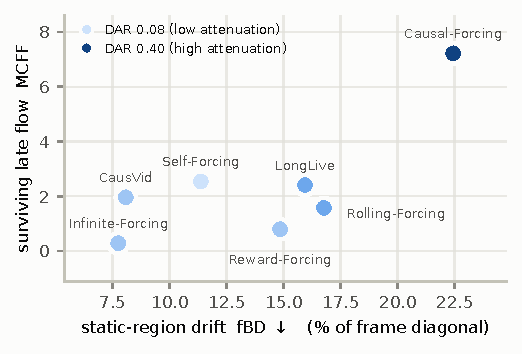
\includegraphics[width=\linewidth]{figures/fig4_operating_regime.pdf}
\caption{\textbf{Operating regimes under native deployment.} Colour encodes the share of dynamic-region flow a global similarity model accounts for. The view exposes trade-offs; it is not a leaderboard.}
\label{fig:regimes_native}
\end{figure}

\subsection{Drift Leakage Changes the Interpretation of Apparent Motion}
\label{sec:results_drift}

The effect is systematic rather than anecdotal. Over the audited systems at 60\,s, VBench Dynamic Degree correlates with SNF-Bench's static-region flow at Spearman $\rho = \SNFddNBF$ (Table~\ref{tab:disagreement}): the systems a generic metric reads as most dynamic are, to a close approximation, the systems whose backgrounds move most. The consequence for ordering is direct. Causal-Forcing ranks \SNFrankCFDD{} of \SNFnPublicTTV{} on Dynamic Degree and \SNFrankCFNBF{} of \SNFnPublicTTV{} on NBF; Infinite-Forcing occupies the mirror position, ranking \SNFrankIFNBF{} on static fidelity and \SNFrankIFDD{} on apparent motion. Read jointly with its magnitudes, Causal-Forcing's DLR of \SNFvalCFDLR{} indicates static-region motion energy almost equal to that of the region intended to move, while its DAR of \SNFvalCFDAR{} indicates that a rigid global model accounts for only part of it---the remainder is non-rigid instability, which a translation-only account would have misdescribed.

\begin{table}[t]
\centering
\small
\begin{tabular}{lcccc}
\toprule
generic metric & fBD & NBF & MCFF & DLR \\
\midrule
VB-DD & +0.75 & +0.93 & +0.89 & +0.36 \\
VB-bg & -0.64 & -0.71 & -0.75 & -0.50 \\
VB-smooth & -0.96 & -0.82 & -0.61 & -0.64 \\
VB-flick & -0.96 & -0.82 & -0.61 & -0.64 \\
\bottomrule
\end{tabular}
\caption{\textbf{Rank disagreement at 60\,s.} Spearman correlation between generic whole-frame metrics and SNF-Bench factors over method-level means. A positive correlation between apparent motion and background flow is the effect the benchmark isolates.}
\label{tab:disagreement}
\end{table}

The supplementary material records every interpretation change meeting three conditions fixed in advance: both measurements are computed on the same outputs, the SNF factor involved passed the validation of Sec.~\ref{sec:validation}, and the rank difference exceeds a fixed threshold rather than reflecting a small ordinal shift. The rule is applied to every audited system, so no qualifying case can be selectively omitted. The analysis is complementary: whole-frame metrics measure what they were designed to measure, and SNF-Bench exposes where that quantity spatially originates.


\subsection{Category and Horizon Dependence}
\label{sec:results_categories}

Aggregates can conceal scene dependence, so all headline numbers are macro-averaged over the \SNFnCategories{} flow-medium categories of Sec.~\ref{sec:benchmark} rather than averaged over prompts directly. This matters: the 60\,s prompt set is \SNFtopCatShare\% channel water, so a prompt-level mean is substantially a measurement of one medium. Complete per-category values appear in the supplementary material, together with the category balance of every track and horizon.

Horizon dependence is read from the per-horizon panels of Table~\ref{tab:t2v_audit}. A useful long-horizon generator should not merely score well at one duration but remain comparatively stable as the horizon grows. The 5\,s tier serves as an initialization sanity check; the 240\,s tier is exploratory and determines no principal conclusion, but it is reported because the ordering it induces is itself evidence about metric behavior under extended rollout.
